% !TEX TS-program = xelatex
% !TEX encoding = UTF-8
\documentclass[12pt,a4paper]{report}
\usepackage{graphicx}
\usepackage[UTF8, heading=true]{ctex}
\usepackage{indentfirst}
\usepackage{amsmath}
\graphicspath{{section/}{figures/}}
\usepackage{tikz}
%\usepackage{CJK}
\usepackage{url}

\setcounter{secnumdepth}{3}
\renewcommand\thesection{\arabic {section}}
\usepackage{float}
\usepackage{subfig}
\usepackage{caption}
\usepackage{lipsum}
\usepackage[unicode, colorlinks=true]{hyperref}

\begin{document}
%%%%%%%%%%%%%%%%%%%%%%%%%%%%%%
%% 封面部分
%%%%%%%%%%%%%%%%%%%%%%%%%%%%%%
\begin{titlepage}
    \centering
    
\includegraphics[width=0.2\textwidth]{sf1.png}\par
    \vspace{1cm}
    
\includegraphics[width=0.8\textwidth]{sf.jpg}\par
    \vspace{0.1cm}
    {\scshape\LARGE Harbin Institute of Technology \par}
    \vspace{1cm}
    {\kaishu\LARGE 面向微系统的图像测试技术课程报告\par}
    \vspace{1.5cm}
    {\huge\bfseries 圆孔图像提取与识别\par}
    \vspace{2cm}
    {\fangsong\Large\itshape 卢XX, 张XX\par}
    \vfill
    {**********, **********}\par
    \fangsong{XX系}

    \vfill
    指导教师	\textsc{王XX}
    \vfill
% Bottom of the page
    {\large \today\par}
\end{titlepage}

\section{引~~~~言}

MEMS技术是近年来随着微电子技术的不断成熟而发展起来的一门新兴的交叉学科。 
其涵盖领域包括光学、机械、电子、计算机等诸多门类。 
随着MEMS技术发展及应用的扩展,对其微细结构的性能及结构的测试要求也日益迫切。 
由于其结构尺度属微纳米量级,因此传统意义的测试技术,几乎无能为力。 
本文针对MEMS装配领域中的目标物识别,通过图象处理处理手段,
利用计算机技术及CCD图像采集,进行微型圆孔的自动图像识别。

\section{设计要求}

\begin{figure}[htb]
    \centering
    \subfloat[A组]{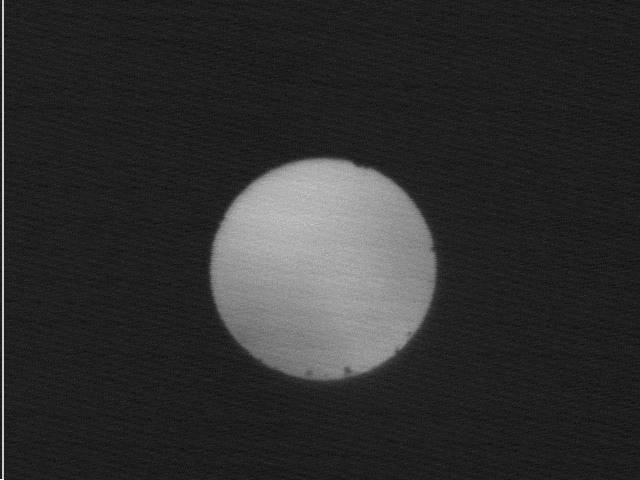
\includegraphics[width = 0.48\linewidth]{A.png}}\hfill
    \subfloat[B组]{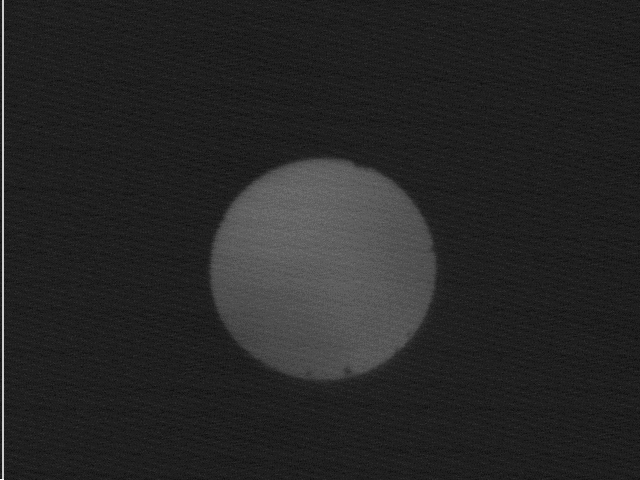
\includegraphics[width = 0.48\linewidth]{B.png}}\\
    \subfloat[C组]{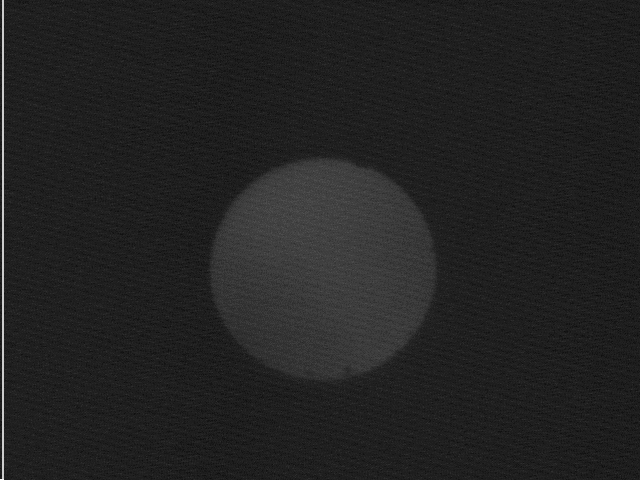
\includegraphics[width = 0.48\linewidth]{C.png}}
    \caption{采集图像}\label{fig:origin}
\end{figure}

图\ref{fig:origin} 为CCD在不同曝光时间内采集到的微型圆孔图像。
要求从图中提取出边缘信息,能够拟合出圆心和半径等参数, 
同时,要求能尽可能多的保留圆上的缺陷等细节信息,
且处理算法应具有一定的兼容性,以便日后能够实际应用。

\section{研究方法}

虽然直接按传统方法难以准确有效地识别此类图像,
但通过对传统方法的分析和组合,尝试出了一种行之有效的处理流程:
\begin{itemize}
    \item 第一步,滤波降噪;
    \item 第二步,二值化处理;
    \item 第三步,边缘检测;
    \item 第四步,提取边缘,拟合圆,计算圆心和半径。
\end{itemize}

这四步基本每一步所用的都是传统算法,通过合理的排列使之得以有效的识别。

\subsection{滤波算法}

根据设计要求,滤波算法的选取应该既能够降低噪声,又可以保持图形的边缘形态。
由于能力限制,最终在程序中提供的滤波算法只有四种:
\begin{itemize}
    \item 均值滤波 - 线性滤波,边缘保持能力差。
    \item 高斯滤波 - 线性滤波,边缘保持能力较差。
    \item 中值滤波 - 非线性滤波,边缘保持能力较好。
    \item 均值平移滤波 - 非线性滤波,边缘保持能力好,但性能较差。
\end{itemize}
这其中,均值滤波基本就是拿来练手的。

\lipsum[1]

\subsection{二值化之阈值分割算法}

二值化本身的算法并没有什么特别的,就是普通的单一阈值分割。
重要的是选取阈值所用的方法。

\lipsum[1]

\subsection{边缘检测算法}

在传统的Canny边缘算法中,边缘检测算子是先于二值化进行的。

\lipsum[1]

\subsection{圆拟合与误差矫正}

\lipsum[1]

\section{程序说明}

\lipsum[1]

\end{document}
